\documentclass[../main/main.tex]{subfiles}

\newdate{date}{16}{10}{2020}


\begin{document}

\marginpar{ \textbf{Lecture 7.} \\  \displaydate{date}. \\ Compiled:  \today.}

To summarize, we have seen that for most real networks it has been showed that the average path length scales as:
\begin{equation*}
  \expval{l} \approx \ln{N}
\end{equation*}
with the logarithm of the number of nodes in the network, not just with the number of nodes. Or in some cases as \( \expval{l} \approx \ln(\ln(N))  \).
How is it possible? A paper which explain it is “Collective dynamics of small world networks” of Watts and Strogatz. Their idea is what is called the \textbf{Watss and Strogatz model}.

\begin{figure}[h!]
\centering
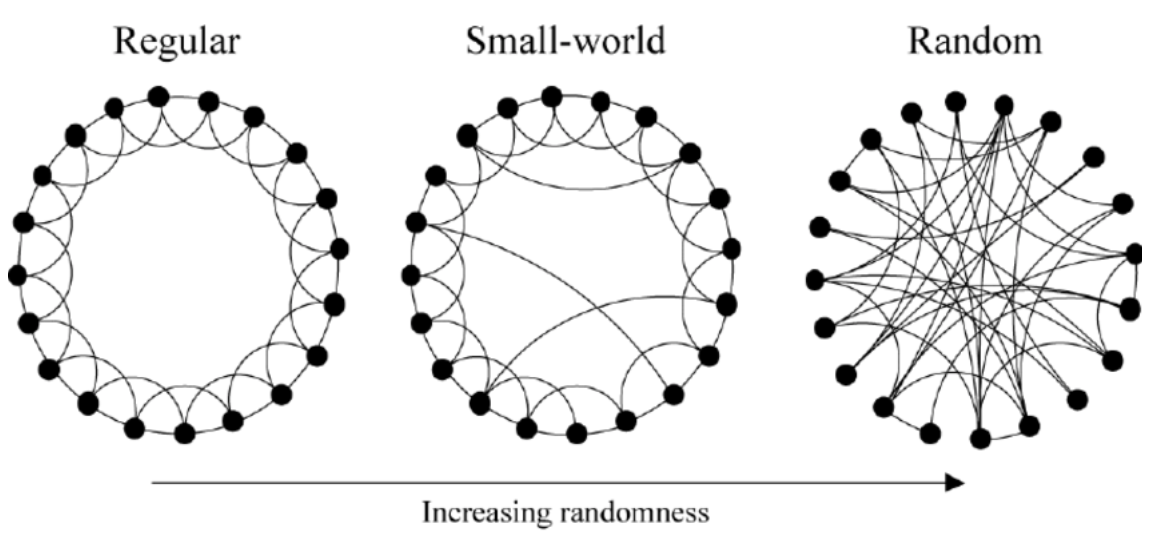
\includegraphics[width=0.7\textwidth]{../lessons/image/07/1.png}
\caption{\label{fig:07_1} Idea of Watts and Strogatz model.}
\end{figure}


Let us focus with the first regular ring in Fig. \ref{fig:07_1} in which we have each node connected with its neighbour in its left and right. The structure is totally regular. If we want to measure the longest distance that we can find in the network we have that:
\begin{equation*}
  \expval{l^{circle}} \sim \frac{N}{4 m}
\end{equation*}
What happens if we just rewire one of the connection? We connect it with a another random nodes in the network as in small-world circle in Fig. \ref{fig:07_1}. What do happen for the distance? Just rewiring one connection reduce the size in an incredible way. If we can control the number of connection with a probability \( p \), what happens is that every time we rewire the connection, the average steps is reduced by a factor 2. If we repeat this process several time we obtain a logarithmic scaling. At the end we obtain a random network which scales as:
\begin{equation*}
  \expval{l} \sim \log{N}
\end{equation*}
It is represented by the random circle in Fig. \ref{fig:07_1}.

\section{Degree distribution over networks}
Now the question is how degrees are distributed over the newtwork. Let us consider a small network, the plot on the left of Fig. \ref{fig:07_2} represents the distribution of the degrees in this small network. How is this quantity distributed in real networks?

\begin{figure}[h!]
\begin{minipage}[c]{0.5\linewidth}
\centering
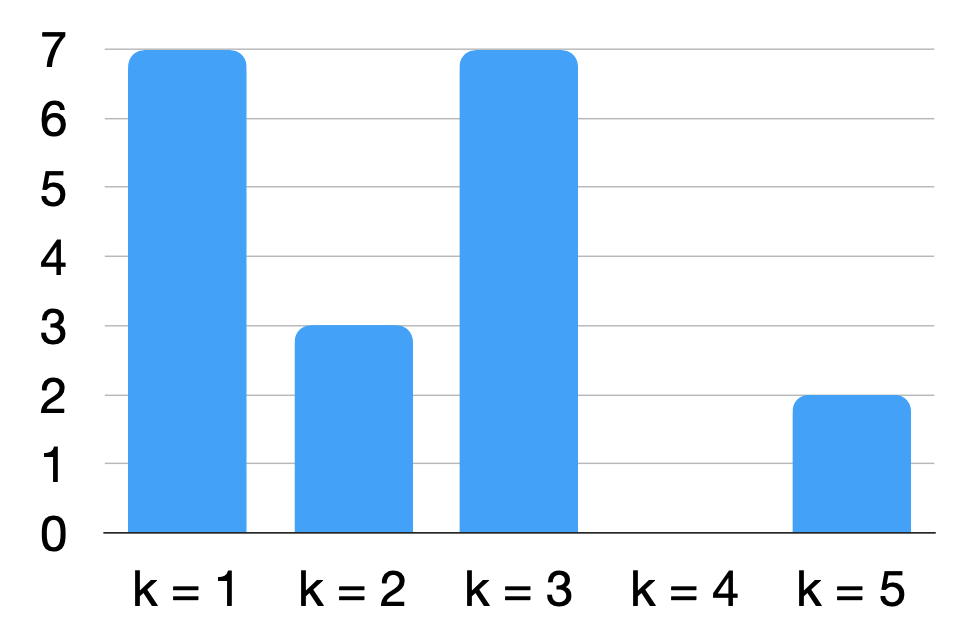
\includegraphics[width=0.8\textwidth]{../lessons/image/07/2.png}
\end{minipage}
\begin{minipage}[]{0.5\linewidth}
\centering
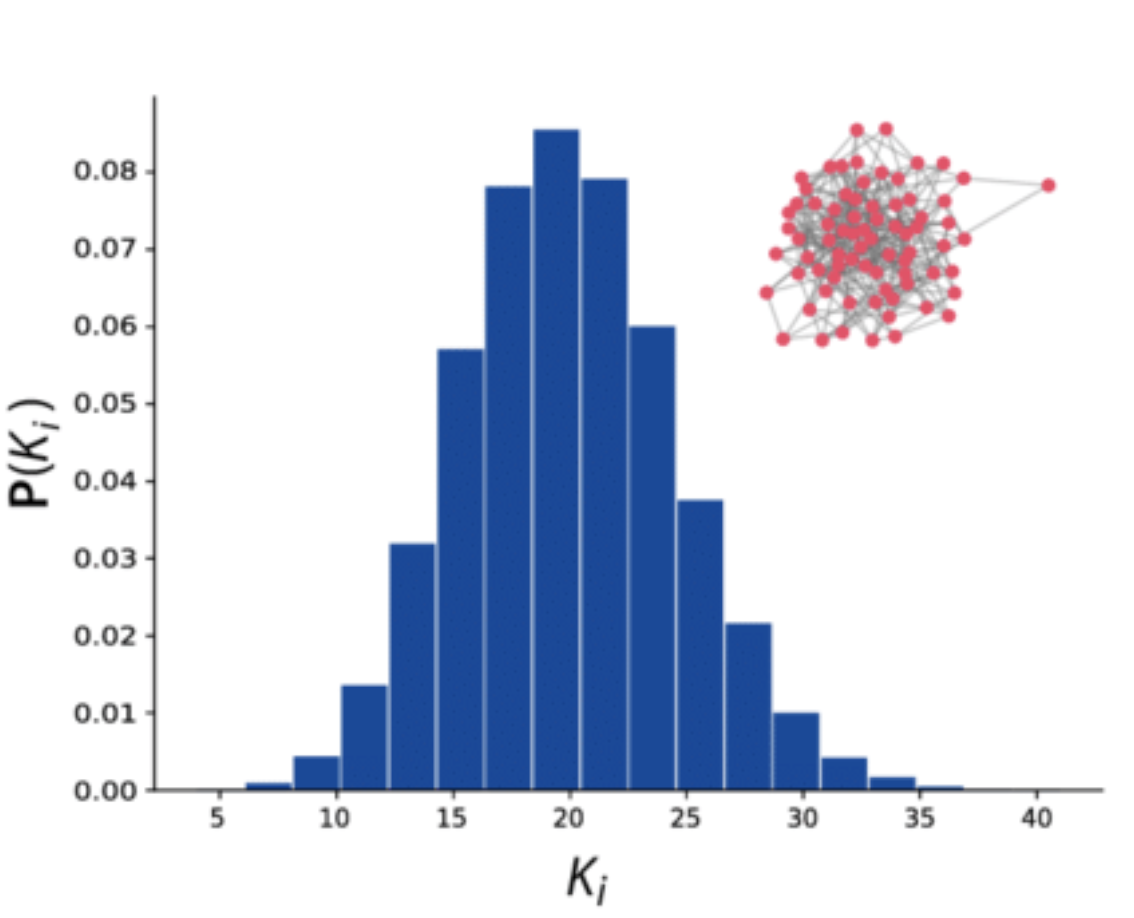
\includegraphics[width=0.8\textwidth]{../lessons/image/07/3.png}
\end{minipage}
\caption{\label{fig:07_2} \textbf{Left:} degree distribution in a small network. \textbf{Right:} degree distribution in a network with random connections. }
\end{figure}

The first assumption that we can make is building the connections at random. Hence, there is no rule behind the degree distribution but a probability distribution as the one on the right of Fig. \ref{fig:07_2}.

\subsection{Erdös and Rényi Model: random graphs}
Let us consider the Erdös and Rényi model which represents the evolution of a graph where links between nodes are drawn at random. In particular, the algorithm for creating such a network is:
\begin{itemize}
\item create an empty graph with $N$ nodes;
\item connect each possible couple of nodes with probability $p$;
\item avoid self-loops and multiple edges.
\end{itemize}
What are the properties of this graph?
Let us consider a graph \( G(N,p) \) where \( N \) are the number of nodes and \( p \) is the probability of connection.
Before 1959 (the year of the publication of Erdös and Rényi's paper) people assumed that connection were regular, hence this is the first time in which random connections are been considered.
If links are drawn at random with probability $p$, the probability that a node has $k$ neighbors $p_k$ is given by a binomial distribution:
\begin{equation}
  p_k = \binom{N-1}{k} p^k (1-p)^{N-1-k}
\end{equation}
The average and variance of such a distribution are:
\begin{equation}
  \expval{k} = p(N-1), \qquad \sigma _k^2 = p(1-p)(N-1)
\end{equation}
As we can see, the average and the variance scales in the same way with the size of the network.
The problem of the last distribution is that it is difficult to be treated analitically when \( N \) increases, indeed:
\begin{equation*}
  \frac{\sigma _k}{\expval{k} } = \sqrt{\frac{1-p}{p(N-1)}} \overset{N \rightarrow \infty }{\longrightarrow } 0
\end{equation*}
which is very narrow as \( N \) increases, so we need a kind of approximation.

Fortunately, for sparse networks we have \( k \ll N \), hence the binomial \( (N,p) \) distribution can be approximated by a Poisson distribution with \( \lambda = p N \). Indeed, since  \( \expval{k} = p(N-1)  \), having \( k \ll N \) implies \( p \ll N \) and thus:
\begin{equation*}
  (1-p)^{N-1-k} \approx e^{(N-1-k) \log (1- \expval{k}/(N-1) )} \overset{N \rightarrow \infty }{\longrightarrow } e^{- \expval{k} }
\end{equation*}
and
\begin{equation*}
  \binom{N-1}{k} \approx \frac{(N-1)^k}{k!}
\end{equation*}
Obtaining:
\begin{equation}
  p_k = e^{- \expval{k} } \frac{\expval{k} }{k!}
\end{equation}
As before, the average and the variance scales in the same way with the size of the network. This is telling us that all the nodes more or less are the same. If we have a bounded variance means that all the nodes have more or less the same degree. That is the point.
In particular, as $p$ is increased the graph undergoes a transition from disconnected to fully connected:
\begin{itemize}
\item if \( N p < 1 \), the graph will almost surely have no connected compontens of size larger than \( O(\log(N)) \);
\item if \( N p = 1 \), the graph will almost surely have a giant component of size \( O(N^{2/3}) \);
\item if \( N p \rightarrow c > 1 \), the graph will almost surely have a giant component comprising a large fraction of the nodes;
\item if \( p < \frac{(1- \varepsilon )\ln N}{N} \), the graph will almost surely contain isolated vertices;
\item if \( p > \frac{(1- \varepsilon )\ln N}{N} \),  the graph will almost surely be connected.
\end{itemize}

\begin{figure}[h!]
\centering
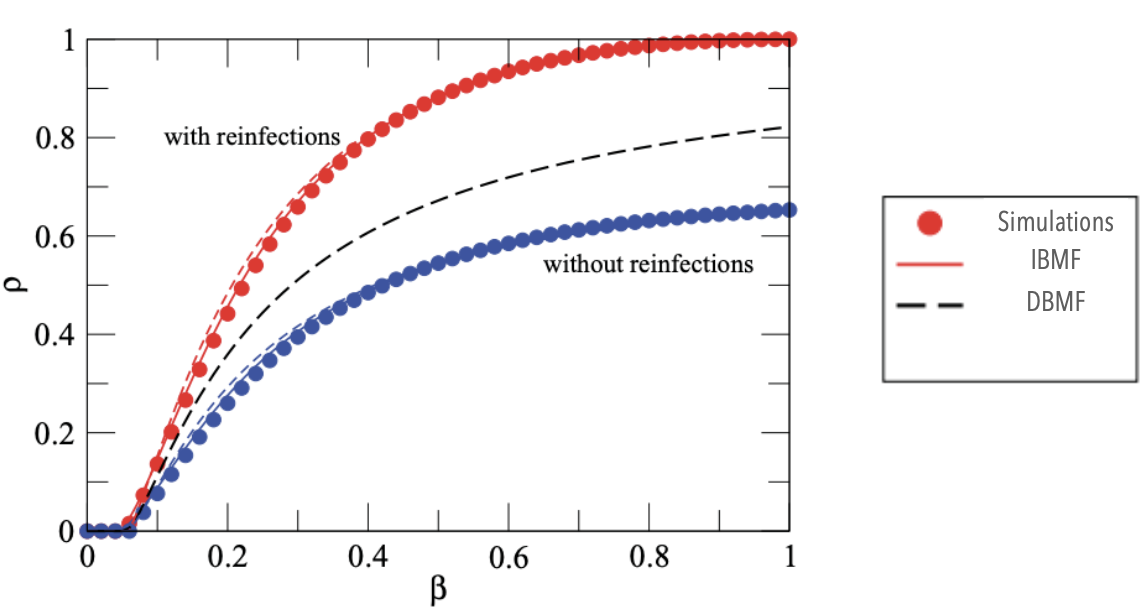
\includegraphics[width=0.8\textwidth]{../lessons/image/07/4.png}
\caption{\label{fig:07_4} Real network of Facebook and Twitter.}
\end{figure}

\subsection{Scale-free networks}

The point now is: what is the degree distribution of real networks? In the last decades we start to have very very complex and large networks. Their structure is nothing like the structure that you see for a random network. In Fig. \ref{fig:07_4} are shown real network of social networks as Facebook and Twitter. All this plots are in log-log scale. We can conclude that most of the networks scales in the same way.
But, what is the form of this connection? Let us consider Fig. \ref{fig:07_4}, the black curve represents the Poissonian distribution that we saw before, and then we plot the power-law (heavy tailed distribution) \( P(k) \sim k^{- \gamma  } \). We see that the Poissonian distribution is not able to reproduce the hetherogeneity you see in the data, while the power-law it is. Hence, in most contexts real networks are highly heterogenous and degrees can vary several orders of magnitude. In particular, the \( \gamma   \) coefficient of the power-law has an important role, since it represents the slope of the curve in log-log scale.
Thus, we have similar structures at different scales, this leads to the concept of scale-free networks. Most real networks have small values of \( \gamma   \), i.e. \( \gamma \le 3 \).


\begin{figure}[h!]
\centering
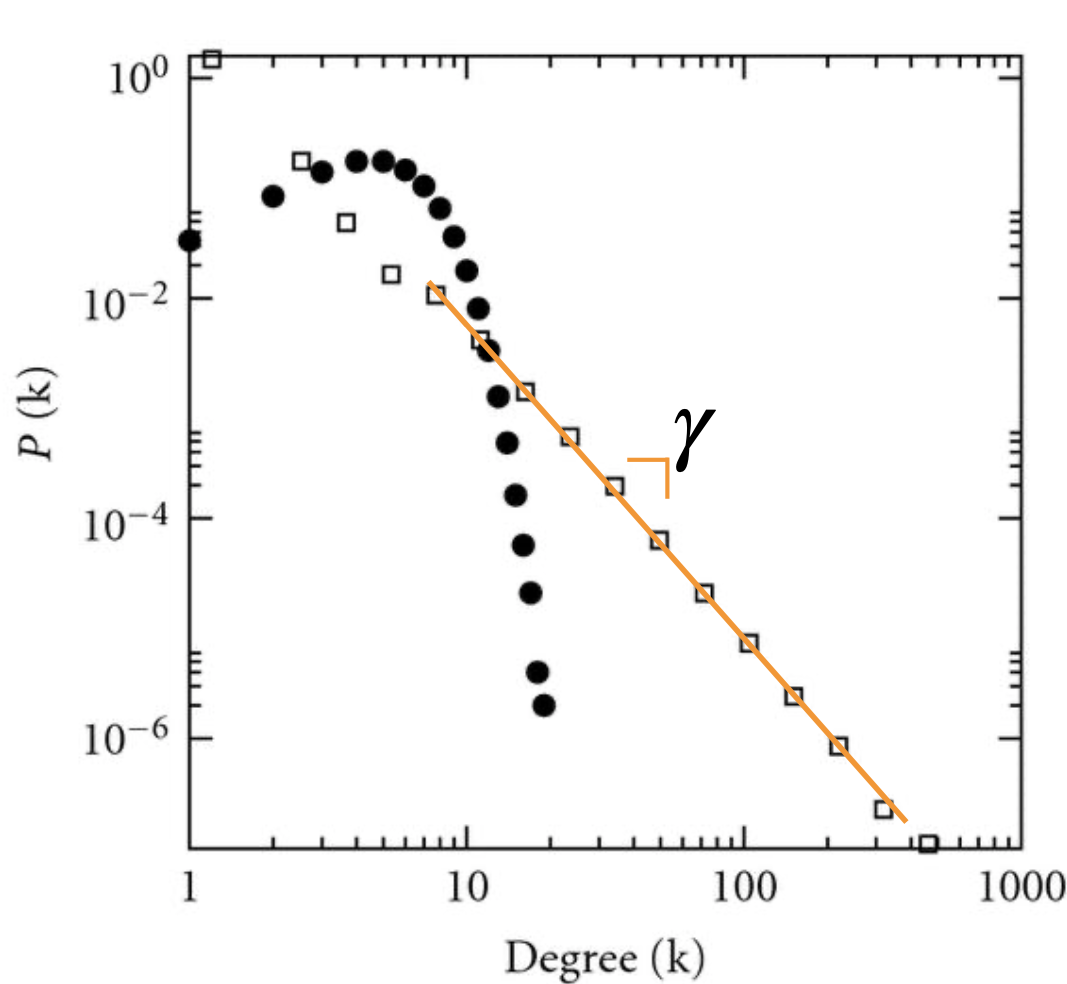
\includegraphics[width=0.7\textwidth]{../lessons/image/07/5.png}
\caption{\label{fig:07_4} Difference between random networks and scale-free networks.}
\end{figure}

Heterogeneous means that most of the nodes have a very low connectivity, less than a random net. However, the probability of having very large degrees is not zero (\textbf{hubs}). Even for small networks you can have large Hubs and this is something we have to take into account for the spreading of diseases since we can have shortcuts for spreading or super-spreaders.

We can study the limiting cases of this scale-free networks. For instance, we can study some of the properties we have seen before, as the average degrees or we can prove how the largest degree scales as the size of the network. Let us consider the power-law:
\begin{equation}
  P(k) = C_0 k^{-\gamma } \qquad \text{with} \quad C_0 = (\gamma -1  ) k_{min}^{\gamma -1 }
\end{equation}
To know how \( k_{max} \) scales with \( N \), we have to study when:
\begin{equation*}
  \int_{k_{max}}^{\infty } P(k) \dd[]{k}  = \frac{1}{N} \quad \rightarrow  \qty(\frac{k_{min}}{k_{max}})^{\gamma -1 } = N
\end{equation*}
Thus, when:
\begin{equation}
  k_{max} = k_{min} N^{\frac{1}{\gamma -1 }}
\end{equation}
The most important thing is that more of the network we have \( \gamma = 2,3  \) as we can see in the previous plot of Fig. \ref{fig:07_3}.

The general \( n^{th} \) moment of the distribution is:
\begin{equation}
  \expval{k^n} = \int_{k_{min}}^{\infty } k^n P(k) \dd[]{k} = \int_{k_{min}}^{\infty }  C_0 k^{n- \gamma  }\dd[]{k}
\end{equation}
It converges only if \( \gamma -1 > n  \). This gives an hint on how the average of the degree scales as the size of the network. This is a very important result. Considering \( \sigma ^2  = \expval{k^2} - \expval{k}^2  \), we have that:
\begin{itemize}
\item if \( \gamma <2  \), both \( \expval{k}  \) and \( \expval{k^2}  \) diverge with \( N \rightarrow  \infty  \);

\item if \( 2 < \gamma < 3  \), the average degree \( \expval{k}  \rightarrow c \) but \( \expval{k^2}  \rightarrow \infty \) as \( N \rightarrow  \infty  \) and \( \sigma ^2 \rightarrow \infty  \).
\end{itemize}
Remember that most real networks have \( \gamma \le 3 \), hence the variance of the degree also diverges and so we have extremely heterogeneous networks not homogeneous ones.
This means that all the models we have been used before in which we assumed that all the people in the population were equal, does not hold anymore.

\subsection{Barabási-Albert Model}
The last thing we need is an algorithm to create a random scale-free network. We can realy on the Barabasi-Albert model. This is the second paper which starts the field. We have to rethink all the models we have been used right now and include these things.

The idea behind this paper is extremely simple. They analized real networks and then they assumed \( P(K) \sim k^{-3} \) in order to create a model to reproduce this behavior.
Their model is based on the concept of growing random networks.
We start with a small number of nodes, at each time-step a new node enters the network and connects with pre-existing nodes but with a preferential attachment.
Hence, at each step the network growth.

The principle behind the preferintial attatchement which is based on a very simple concept: rich get richer. The more connected a node is, the more likely it is to receive new links. The probability to attract a new link at time $t$ proportional to degree at time $t$:
\begin{equation}
  \Pi (k_i) = \frac{k_i}{\sum_{j}^{} k_j }
\end{equation}
In the case of influencers, if I have a lot of followers the probability of increase my connections is increasing too. Actually, this idea is not even so new and it is something we have been known. This model hence is just a modification of the Price model: if I published a paper and someone think that it is interesting, more attention I get more attention I will get in the future.


So, I am drawing the link at random but not uniformely. Let us briefly summarize the main steps of the algorithm:
\begin{itemize}
\item we start with a clique of \( m_0 \) nodes;
\item at each time step \( t \), we add a new node to the network;
\item we create $m$ (i.e. $m=2$) links between the new node and the existing ones according to the preferential attachment (remember to update the connection probability after each link);
\item repeat until size $N$ is reached.
\end{itemize}
In particular, let us consider Fig. \ref{fig:07_5}. We start with a small number of nodes connected in a link. In the first time step I am gonna adding a new node, and I am gonna connectecting to the other nodes. Let us assume that every time I add a node, I am adding two links. I calculate the probability of getting a new node which in this case is equal for all the nodes. Then I pick up one at random and I connect to it. Then I have to update the probabilities. We see that the node on the left got an higher probability of getting new connections. Then I start with a ned node untile size \( N \) is reached.

\begin{figure}[h!]
\begin{minipage}[c]{0.48\linewidth}
\centering
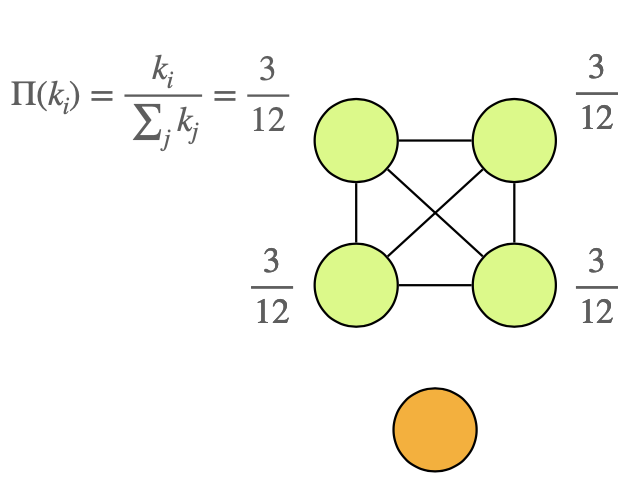
\includegraphics[width=0.8\textwidth]{../lessons/image/07/6.png}
\end{minipage}
\( \longrightarrow  \)
\begin{minipage}[]{0.48\linewidth}
\centering
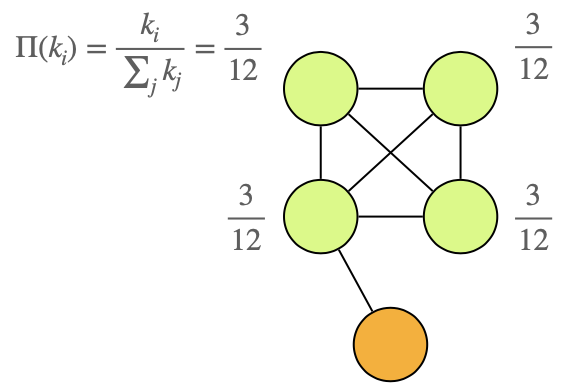
\includegraphics[width=0.8\textwidth]{../lessons/image/07/7.png}
\end{minipage}
\caption{\label{fig:07_5} Example of Barabási-Albert algorithm.}
\end{figure}

This algorithm is able to create netowrks with some interesting properties. The simple idea is that the degree distribution is:
\begin{equation*}
  P(k) = \frac{2 m (m +1)}{k(k+1)(k+2)} \sim k^{-3}
\end{equation*}
for large \( k \), where \( m \) is the number of links you are adding at each step (this is a parameter which drives you the minimal degree of the network).
We obtained that we obtained \( \gamma =3  \) independent from \( m \) and \( m_0 \). Hence, the maximum degree of the network scales as \( k_{max} \sim N^{1/2} \). Moreover, we have that \( \expval{k} \rightarrow c \), but \( \expval{k^2} \rightarrow \infty   \) with \( N \), as before.
The length of the network is:
\begin{equation*}
  \expval{l} \sim \frac{\ln (N)}{\ln (\ln (N))}
\end{equation*}
hence we have small-world.










\chapter{Epidemic Spreding on Networks}

\subsection{SIS model in a network}

The idea is that we pass from the classical well-mixed population to the contact networks. So we assume that we have some sort of connection between individuals. The idea is that:
\begin{itemize}
\item all individuals are equivalent;
\item individuals do not interact at random: friends, family and so on. You have somehow constraing how the disease will spread. The fact that we have repeated contacts has strong effect on the dynamics.
\end{itemize}
Let us try to build a general model for a general network. For doing that the idea is, let us start with the SIS dynamics and defining a binary variables in the sense that can only have two values: 0 if it is susceptibòe and 1 if it is infected. We define another variable \( \rho (i,t) \) which represent the probability of that node \( i \) is infected at time \( t \). So from here, I can write a general equation for the SIS in a nwtork:
\begin{equation*}
  \dv{}{t} \rho (i,t) = \overset{\text{Recovery}}{- \mu  \rho (i,t)} + \overset{\text{Infection}}{\beta \sum_{j}^{} A_{ij} \text{Prob} [\sigma _i (t) = 0, \sigma _j (t ) =1 ]   }
\end{equation*}
The problematic part is the probability which is... we have to find an expression for it. Since we ae in a network, the probability of being ifnected depends on my neighbours. I have to follow the entire chain of connection. No closed form, it depends on the three nodes probability and so on... I have to follow the entire network if I want to know what is gonna happening.
We have to write down the entire time evolution of the system.

The idea is that since I will gonna have this chain of probability, I need to cut down this chain at some point. So at some point I need a closure of my equation. I am not taking into account all the structure of the network, but at some point I will the the average. We need some sort of approximation for this probability. After that we will be able to solve the problem.
In physics this are called mean-field approximation, since I am not able to solve the many body problem at a certain point I will consider a random field which acts on the entire system and at some point I will consider the average effects on the system.

What happens is that I am susbtituting in some way this probability \( \text{Prob} [\sigma _i (t) = 0, \sigma _j (t ) =1 ]  \) with some average probability.
Obviously, depengin on the assumption we are making for this approximation we will obtain different results. If I am assuming that the network is homoegenous (all the nodes are equal) I have a mean-field, if it is heterogeneous I will have more equations but I will have a more reliable approximation of the system.

Coarse graining level.
The distinction can be also in the level I will adopt this approximation. We can have degree based mean field theories in which we assume that all the nodes of the same degree are equal. While individual bases mean field means that all the nodes are different and that I will take individual connections between individuals. The probability of having the disease for a node can be different depending on different factors...

Where to cut the level? In individual level or pair approximation?

Let us start with the simplest approximation.

\subsection{Homogeneous networks}
The important thing is that the variance and standard deviation is bounded. I am assuming that all the nodes are equal. I can forget about phase, the position of the node on the network does not matter anymore because the nodes are equal.

I am gonna make the mean field at the individual level: I am approximation the probability \( \text{Prob} [\sigma _i (t) = 0, \sigma _j (t ) =1 ] \) (one being infected and the other one supsceptible) are statistically independent. Hence, I can decompose this one with a product of individual probability \( \text{Prob} [\sigma _i (t) = 0] \cdot \text{Prob} [\sigma _j (t ) =1 ] \).
I define:
\begin{equation*}
  \rho (t) = \text{Prob} [\sigma (t)=1]
\end{equation*}
If we put everything togheter, we get the equation:
\begin{equation*}
  \dv{\rho }{t}
\end{equation*}
which looks quite familiar, where we have \( \sum_{j}^{} A_{ij}   \) which is the degree of the network.
We get exactly the same expression that we got before for well-mixed population. This is important that actually what are you doing is that all the nodes are statistically independent. I am recovery exactly this result. When I was consider well-mixed population, I assumed that the probabilities where exaxtly statistically independent. Now, this is just an approximation.

All the calculation that we get are gonna hold for this thing. In the labs you will see when this assumption breaks down.

\subsection{Heterogenous netowrks}





\end{document}
